\documentclass[./main.tex]{subfiles}
\begin{document}
\chapter{Particle orbit pusher algorithms}
\vspace{-0.5cm}
This chapter is dedicated to the implemented algorithms for finding the first intersection of particle orbits with the tetrahedral cell boundaries in the grids that were previously introduced. Here, a particle can either start at an arbitrary position inside a given tetrahedron or directly at a face of a tetrahedron through which it enters. These routines efficiently compute the next exiting position of the particle through the tetrahedron and the associated flight time of the trajectory. Since this procedure can be thought of as a pushing of the particle orbit through the tetrahedron, the implemented routines are denoted $pusher$-routines. On a sidenote, the fact that both position and time are obtained directly by the approaches used in the pusher routines, a box counting scheme can easily be implemented for future applications, allowing for a very efficient approximation of particle distribution functions, which in turn are a necessary part for possible future computations of kinetic plasma equilibria. The focus of the pusher routines lies, however, not only on the computation of the trajectory and the calculation of the next intersection but rather on finding a numerically inexpensive scheme that allows to save computational cost while reliably yielding accurate results for the exiting position. In the diploma thesis of M. Eder \cite{Eder_DA}, a prior version of the presented pusher routine was discussed in great detail, this routine was named \texttt{pusher\_tetra\_orb}. Due to new insights and structural limiations of the previous code, this code was refactored and extended in cooperation with M. Eder. The resulting code was named \texttt{pusher\_tetra\_orbit}, an overview of the code is given below, however, due to large similarities with the previous approach discussed in \cite{Eder_DA}, the new route will be presented in less detail. Apart from this routine, a second routine named \texttt{pusher\_tetra\_analytic} was implemented based on the previously derived polynomial expansion of the particle orbit. While the results are in theory equivalent for both pushing routines, the approaches are completely independent and thus may vary in both computational efficiency and numerical accuracy, depending on up to which order the analytical expansion of the orbit is computed. Furthermore, for starting a particle at a given position without knowing to which tetrahedron it belongs, an additional routine \texttt{find\_tetra} was constructed to find the corresponding tetrahedron index to start a calculation.
\section{Pusher routine \texttt{pusher\_tetra\_orbit}}
\label{sec:NumericalPusher}
As discussed, the pusher subroutine \texttt{pusher\_tetra\_orbit} computes the position and time where the particle trajectory first exits a given current tetrahedron. In reality, however, the occurring problem is not only to directly compute the orbit of a single tetrahedron passing, but rather to let a particle start at a position in space and trace its orbit for a defined time. For such a problem one can construct a wrapping routine \texttt{orbit\_timestep\_3dgeoint} which is given the initial conditions of the particle and iteratively calls the pusher subroutine \texttt{pusher\_tetra\_orbit} until the set time is reached. Since generally the set flight time of the particle will lead to an orbit position inside the final tetrahedron, the remaining time of the trajectory must also be given to the pusher routine. The pusher routine then computes the time it takes until the particle exits the current tetrahedron and compares this value to the remaining time of the orbit integration step which was given to the wrapper routine. In case the time it takes to leave the tetrahedron is smaller than the remaining time, the pushing is computed, then the remaining time is reduced by this value and the next pushing through the adjacent tetrahedron is started. In case there is not sufficient time to complete the pushing, the orbit is instead integrated up to the value of the orbit parameter \texttt{tau} corresponding to the remaining time, leading to an arbitrary final position inside the tetrahedron. The code structure of the wrapping routine \texttt{orbit\_timestep\_3dgeoint} and the components of the module \texttt{pusher\_tetra\_orbit\_mod} is given in figure \ref{fig:Codestructure_Pusher_tetra_orbit}. 

\begin{figure}[h!]
	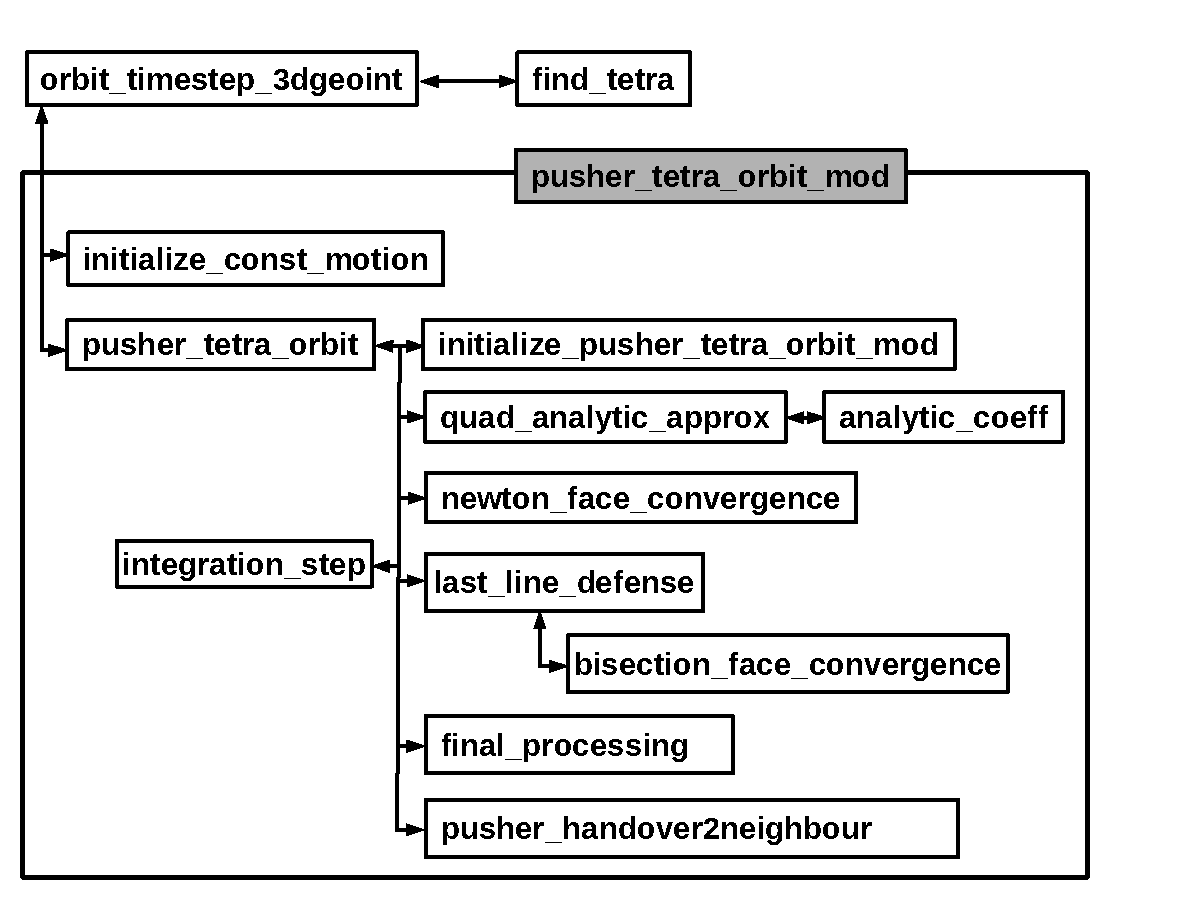
\includegraphics[width=1\textwidth]{figures/pusher_tetra_orbit.pdf}
	\caption{Code structure of \texttt{pusher\_tetra\_orbit\_mod} and associated subroutine}
	\label{fig:Codestructure_Pusher_tetra_orbit}
\end{figure}

Due to this wrapping routine, one can directly start the computation of a single particle orbit for a given flight time by calling subroutine \texttt{orbit\_timestep\_3dgeoint} with arguments \texttt{(x,vpar,vperp,t\_step,boole\_initialized,ind\_tetr,iface)}. This list of parameters is explained in tab. \ref{tab:input_orbit_timestep}.

\begin{centering}
	\begin{table}[H]
		
		\caption{Parameter overview for wrapper subroutine \texttt{orbit\_timestep\_3dgeoint}, defines initial conditions and duration of particle motion, orientations of velocities are taken with respect to the orientation of the magnetic field $\vec{B}$.}
		\begin{tabular}{|l|l|l|}
			\hline
			\rowcolor{lightgray}
			Data type&Name&Description \\
			\hline
			\texttt{double precision,}&\texttt{x}&particle position\\
			\texttt{dimension(3),intent(inout)}&&\\
			\hline
			\texttt{double precision,}&\texttt{vpar}&parallel velocity\\
			\texttt{intent(inout)}&&\\
			\hline
			\texttt{double precision,}&\texttt{vperp}&perpendicular velocity\\
			\texttt{intent(inout)}&&\\
			\hline
			\texttt{double precision,intent(in)}&\texttt{t\_step}&defined flight time\\
			\hline
			\texttt{logical,intent(inout)}&\texttt{boole\_initialized}&sets initialization of\\
			&&constants of motion\\
			\hline
			\texttt{integer,intent(inout)}&\texttt{ind\_tetr}&tetrahedron index \\
			&&at position \texttt{x}\\
			
			\hline
			\texttt{integer,intent(inout)}&\texttt{iface}&index of face if \texttt{x} lies \\
			&&on face, 0 otherwise\\
			\hline
		\end{tabular}
		\label{tab:input_orbit_timestep}	
	\end{table}
\end{centering}

\subsection{Initializing constants of motion}
In figure \ref{fig:Codestructure_Pusher_tetra_orbit}, one can see the code diagram which gives an overview of the different subroutines. When starting a calculation in \texttt{orbit\_timestep\_3dgeoint} for a defined step length, the subroutine that is called first is \texttt{initialize\_const\_motion} which sets the constants of motion for the given initial conditions. These constants of motion are \texttt{E\_tot}, \texttt{perpinv} and \texttt{perinv2} which denote the total energy $E$, the negative perpendicular adiabatic invariant $-J_\perp$ and the squared value thereof, respectively. Since these quantities are saved with attributes \texttt{public,protected}, the subroutine \texttt{initialize\_const\_motion} must be saved within the current module \texttt{pusher\_tetra\_orbit\_mod}, otherwise it would not be allowed to set the values. The constants of motion will retain their set values for a number of tetrahedral pushings until the next time step is executed. Usually, between time steps collision events will occur when performing Monte Carlo simulations, as a consequence the constants of motion may change and have to be defined anew.


\subsection{Particle pushing algorithm}
For a given time step, after initializing the constants of motion, the subroutine \texttt{pusher\_tetra\_orbit} is called with the initial conditions of the current pushing. At the end of the subroutine execution it returns the new starting conditions for the next pushing as well as the remaining time of the current step. An overview of the call parameters of the subroutine is given in tab. \ref{tab:input_pusher_tetra_orbit}.

\begin{centering}
	\begin{table}[H]
		
		\caption{Parameter overview for \texttt{pusher\_tetra\_orbit}}
		\begin{tabular}{|l|l|l|}
			\hline
			\rowcolor{lightgray}
			Data type&Name&Description \\
\hline
\texttt{integer,}		&\texttt{ind\_tetr\_inout}&current tetrahedron index\\
\texttt{intent(inout)}		&&\\
\hline
\texttt{integer,}		&\texttt{iface}&current face index of tetrahedron\\
\texttt{intent(inout)}		&&where orbit converged, 0 if not converged\\
\hline
\texttt{double precision,}			&\texttt{x}&current particle position in \textit{global}\\
\texttt{dimension(3),}			&& coordinates, i.e. not with respect\\
\texttt{intent(inout)}			&& to the first node of a tetrahedron\\
\hline
\texttt{double precision,}			&\texttt{vpar}&parallel velocity of the\\
\texttt{intent(inout)}			&& particle with respect to $\textbf{B}$\\
\hline
\texttt{double precision,}			&\texttt{z\_final}& final particle position in \textit{local} coordinates,\\
\texttt{dimension(3),}				&&  needed for calculation of the flux tube \\
\texttt{intent(out)}				&& volume used in another application\\
\hline
\texttt{double precision,}			&\texttt{t\_remain\_in}& remaining time of the current integration\\
\texttt{intent(in)}			&& step, which consists of many pushings\\
\hline
\texttt{double precision,}			&\texttt{t\_pass}&flight time of the current pushing step\\
\texttt{intent(out)}			&&\\
\hline
\texttt{logical,}			&\texttt{boole\_t\_finished}&boolean stating if the remaining step time \\
\texttt{intent(out)}			&&has been reached in the current pushing\\
\hline
\texttt{integer,}			&\texttt{iper\_phi}&+1,-1 if the particle travels through the\\
\texttt{intent(out)}			&& $\varphi=0$-plane in $-\varphi,+\varphi$ direction, \\
			&&0 otherwise\\
\hline
		\end{tabular}
		\label{tab:input_pusher_tetra_orbit}

	\end{table}
\end{centering}

\subsubsection{Initialize pusher} 
In the \texttt{pusher\_tetra\_orbit} subroutine, first an initializer subroutine \texttt{initialize\_push}
\texttt{er\_tetra\_orbit\_mod} is called. Here, the initial conditions are used to compute the coefficients $a^i_l, b^i$ for the ordinary differential equation set \ref{standeqset}, representing the equations of motion \cite{Eder_DA}.
\subsubsection{Initial guess of exit plane}
Now, that the necessary components of the ODE set \ref{standeqset} have been initialized, the next occurring orbit intersection needs to be computed by the pusher routine. Since this must be done efficiently, a numerically inexpensive approximative quadratic solution is first evaluated by subroutine \texttt{quad\_analytic\_approx} to compute the guess for the orbit parameter \texttt{tau} at the first intersection of the particle trajectory with the cell boundary. Based on the result for the orbit parameter \texttt{tau}, an integration step is performed for the given step length using an RK4 solver, this integrator type is explained in more detail in appendix \ref{chap:AppendixB}. The RK4 integrator subsequently returns the evaluated position for the specified value for \texttt{tau}. In general, due to inaccuracies in the approximation, this value does not correspond to a converged orbit position. 
On a sidenote, in the context of the pusher routine, converged simply means that the particle position is within a defined convergence distance to a given tetrahedral plane. This distance is given by $10^{-10}$ times the normal distance of the first vertex within a given tetrahedron to its opposing cell boundary spanned by vertices 2,3 and 4. In addition, the normal velocity, which can also be computed from the output of the RK4 step, must have a negative sign in order for the convergence to be valid. The negative sign merely states that the particle is flying outwards of the tetrahedron. If there particle flew inwards, it would therefore not be accepted. 
Now, since the orbit position is generally not yet converged after the quadratic approximation, one next applies Newton's method for the face convergence by calling the subroutine \texttt{newton\_face\_convergence}. A detailed description of this approach is given by M. Eder \textit{et al} \cite{Eder_DA}. 






\newpage
\section{Pusher routine \texttt{pusher\_tetra\_orbit\_analytic}}
\label{sec:AnalyticPusher}
\emph{Implementation of analytic pusher from analytical solution}
\newpage
\section{Search routines for tetrahedra with starting points}

\emph{depending on the level of detail, the numerical pusher and the analytic pusher can be anything from a short overview to a lengthy description}
\end{document}




%
%
%
%\documentclass[./main.tex]{subfiles}
%\begin{document}
%\chapter{Particle pusher algorithms}
%\vspace{-0.5cm}
%This chapter is dedicated to the implemented algorithms for finding the first intersection of particles with the tetrahedral cell boundaries in the grids that were previously introduced. Here, a particle can either start at an arbitrary position inside a given tetrahedron or directly at a face of a tetrahedron through which it enters. These routines efficiently compute the next exiting position of the particle through the tetrahedron and the associated flight time of the trajectory. Since this procedure can be thought of as a pushing of the particle orbit through the tetrahedron, the implemented routines are denoted $pusher$-routines. On a sidenote, the fact that both position and time are obtained directly by the approaches used in the pusher routines, a box counting scheme can easily be implemented for future applications, allowing for a very efficient approximation of particle distribution functions, which in turn are a necessary part for possible future computations of kinetic plasma equilibria. The focus of the pusher routines lies, however, not only on the computation of the trajectory and the calculation of the next intersection but rather on finding a numerically inexpensive scheme that allows to save computational cost while reliably yielding accurate results for the exiting position. In the diploma thesis of M. Eder \cite{Eder_DA}, a prior version of the presented pusher routine was discussed in great detail, this routine was named \texttt{pusher\_tetra\_orb}. Due to new insights and structural limiations of the previous code, this code was refactored and extended in cooperation with M. Eder. The resulting code was named \texttt{pusher\_tetra\_orbit}, an overview of the code is given below, however, due to large similarities with the previous approach discussed in \cite{Eder_DA}, the new route will be presented in less detail. Apart from this routine, a second routine named \texttt{pusher\_tetra\_analytic} was implemented based on the previously derived polynomial expansion of the particle orbit. While the results are in theory equivalent for both pushing routines, the approaches are completely independent and thus may vary in both computational efficiency and numerical accuracy, depending on up to which order the analytical expansion of the orbit is computed. Furthermore, for starting a particle at a given position without knowing to which tetrahedron it belongs, an additional routine \texttt{find\_tetra} was constructed to find the corresponding tetrahedron index to start a calculation.
%\section{Numerical pusher \texttt{pusher\_tetra\_orbit}}
%\label{sec:NumericalPusher}
%For given initial values the subroutine \texttt{pusher\_tetra\_orbit(ind\_tetr\_inout,iface,}
%\texttt{x,vpar,z\_final,t\_remain\_in,t\_pass,boole\_t\_finished,iper\_phi)} computes first of all the position and time where the particle trajectory first leaves a tetrahedron. Apart from position and time, further quantities are evaluated to enable a subsequent calculation of the pushing through the adjacent tetrahedron where the particle enters without extra precomputations. An overview of the call parameters of the subroutine is given in tab.  
%
%\begin{centering}
%	\begin{table}[H]
%		
%		\caption{Parameter overview for \texttt{pusher\_tetra\_orbit}}
%		\begin{tabular}{|l|l|l|}
%			\hline
%			\rowcolor{lightgray}
%			Data type&Name&Description \\
%\hline
%\texttt{integer,}		&\texttt{ind\_tetr\_inout}&current tetrahedron index\\
%\texttt{intent(inout)}		&&\\
%\hline
%\texttt{integer,}		&\texttt{iface}&current face index of tetrahedron\\
%\texttt{intent(inout)}		&&where orbit converged, 0 if not converged\\
%\hline
%\texttt{double precision,}			&\texttt{x}&current particle position in \textit{global}\\
%\texttt{dimension(3),}			&& coordinates, i.e. not with respect\\
%\texttt{intent(inout)}			&& to the first node of a tetrahedron\\
%\hline
%\texttt{double precision,}			&\texttt{vpar}&parallel velocity of the\\
%\texttt{intent(inout)}			&& particle with respect to $\textbf{B}$\\
%\hline
%\texttt{double precision,}			&\texttt{z\_final}& final particle position in \textit{local} coordinates,\\
%\texttt{dimension(3),}				&&  needed for calculation of the flux tube \\
%\texttt{intent(out)}				&& volume used in another application\\
%\hline
%\texttt{double precision,}			&\texttt{t\_remain\_in}& remaining time of the current integration\\
%\texttt{intent(in)}			&& step, which consists of many pushings\\
%\hline
%\texttt{double precision,}			&\texttt{t\_pass}&flight time of the current pushing step\\
%\texttt{intent(out)}			&&\\
%\hline
%\texttt{logical,}			&\texttt{boole\_t\_finished}&boolean stating if the remaining step time \\
%\texttt{intent(out)}			&&has been reached in the current pushing\\
%\hline
%\texttt{integer,}			&\texttt{iper\_phi}&+1,-1 if the particle leaves through the\\
%\texttt{intent(out)}			&& $\varphi=0$-plane in $-\varphi,+\varphi$ direction, \\
%			&&0 otherwise\\
%\hline
%		\end{tabular}
%		\label{tab_input_magdata}	
%	\end{table}
%\end{centering}
%
%
%\newpage
%\section{Analytic pusher \texttt{pusher\_tetra\_orbit\_analytic}}
%\label{sec:AnalyticPusher}
%\emph{Implementation of analytic pusher from analytical solution}
%%\newpage
%\section{Search routine for tetrahedra with starting points}
%
%\end{document}